\documentclass[a4paper]{report}
% \documentclass{report}
\usepackage[utf8]{inputenc}
\usepackage{amsmath}
\usepackage{esint}
\usepackage{tabstackengine}
\usepackage[colorlinks,linkcolor=blue]{hyperref}
\usepackage{xeCJK}
\usepackage{caption}
\usepackage{stackengine}
\usepackage{graphicx}
\graphicspath{ {../resources/figure/mc/} }
\usepackage{float}
\usepackage{amsmath}
\usepackage{ulem}
\usepackage{amsfonts}
\usepackage{blkarray}
\usepackage{enumitem}
\setlist[1]{itemsep=-5pt}
\usepackage{subcaption}
\usepackage{multirow}
\usepackage{tikz}
\usetikzlibrary{calc}
\usepackage{pgfplots}
\usepackage{mathrsfs}
\usepackage{minted}
\usepackage{booktabs}
\usepackage{diagbox}
\pgfplotsset{compat=1.17}
\usetikzlibrary{shapes,arrows,positioning}
\captionsetup[table]{skip=10pt}

%%%% 下面的命令重定义页面边距,使其符合中文刊物习惯 %%%%
\addtolength{\topmargin}{-54pt}
\setlength{\oddsidemargin}{0.63cm}  % 3.17cm - 1 inch
\setlength{\evensidemargin}{\oddsidemargin}
\setlength{\textwidth}{14.66cm}
\setlength{\textheight}{24.00cm}    % 24.62


% 段首不缩进
\setlength{\parindent}{0pt}
%%%% 下面的命令设置行间距与段落间距 %%%%
\linespread{1.2}
% \setlength{\parskip}{1ex}
\setlength{\parskip}{.5\baselineskip}

\def\rlwd{.5pt} \def\rlht{2.2ex} \def\rldp{.5ex}
\def\mydiv#1{~%
  \rule[-\rldp]{\rlwd}{\rlht}%
  \setbox0=\hbox{~#1}%
  \stackunder[\dimexpr\rldp-\rlwd]{~#1}{\rule{\wd0}{\rlwd}}%
}

\title{comm_principle}
\author{Crosstyan}
\date{Dec 2020}


\begin{document}
\tableofcontents
\chapter{Introduction}
\section{Features}
\begin{itemize}
	\item 移动通信必须利用无线电波进行信息传输
	\item 移动通信是在复杂的干扰环境中运行的
	\item 移动通信可以利用的频谱资源非常有限, 而移动通信业务量的需求却与日俱增
	\item 移动通信系统的网络结构多种多样, 网络管理和控制必须有效
	\item 移动通信设备(主要是MS) 必须使用在移动环境中使用
\end{itemize}
\section{常见的移动通信系统}
\begin{itemize}
	\item 无线电寻呼系统 (BB机)
	\item 蜂窝移动通信系统 (模拟1G 见\ref{sec:1g}, 2G......)
	\item 无绳电话系统 (小灵通)
	\item 集群移动通信系统 \ref{sec:truck}
	\item 移动卫星通信系统
	\subitem ARIES (CDMA), IRIDIUM(TDMA), TELEDESIC, ELLIPSO BOREALIS......
	\item 分组无线网
	\subitem 利用无线信道进行分组交换的通信网络. 
\end{itemize}
\section{The First Generation}
\label{sec:1g}
1G和2G或其他数据蜂窝的明显区别是\textbf{移动交换中心}\ref{sec:msc} (即MSC)

1G蜂窝无线电话系统采用的调制技术是\textbf{FM}

TACS是1G的模拟蜂窝移动通信系统,是英国标准
\begin{itemize}
	\item AMPS\footnote{Advanced Mobile Phone System​} (America)
	\item TACS\footnote{Total Access Communication System} (England)
	\item NMT-450 (Europe)
	\item NMT-900 (Europe)
	\item C-450 (German)
	\item NTT (Japan)
\end{itemize}


\section{Trunked radio system}
\label{sec:truck}
集群, 采用的基本技术是「频率共用技术」, 通常使用半双工. 

\begin{itemize}
	\item 把一些各部门分散建立的专用通信网集中起来, 统一建网和管理
	\item 改进频道共用的方式. 移动用户在通信的过程中, 不是固定地占用某一个频道, 而是按下「PTT (Press To Talk)」, 才占用一个频道. 
\end{itemize}

尽可能地提高系统的频率利用率, 以便在有限的频段内为更多用户服务. 
\subsection{Message Trunking}
消息集群
\subsection{Transmission Trunking}
传输集群
\subsection{Quasi Transmission Trunking}
准传输集群. \textbf{综合传输效果最好}
\subsection{标准}
\subsubsection{TETRA}
使用TDMA, $\pi/4$-QDPSK
\subsubsection{iDEN}
摩托罗拉. 



\chapter{Modulation}
\section{Introduction}
\paragraph{移动通信环境中,选择和设计数字调制时应着重考虑调制信号的}
抗干扰噪声、频谱利用高、可实现
\paragraph{应从哪些因素考虑移动信道的影响呢}信道衰落、信道带宽、信道干扰噪声
\paragraph{调频的解调方法是}采用鉴频器和微分器分离信号
\paragraph{研究移动通信的电波传播特性的关键是移动信道模型建立,一般建立信道的方法有}理论分析模型、实测数据统计模型、半分析模型
\paragraph{数字调制可以分成线性调制技术和恒包络调制技术,属于线性调制技术}BPSK、QPSK、多电平PSK、$\pi$/4-DQPSK

\paragraph{研究一种调制解调技术的主要内容}
\begin{itemize}
	\item 调制的原理及实现方法
	\item 已调信号的频谱特性
	\item 解调的原理和实现方法
	\item 解调后的信噪比或误码率性能
\end{itemize}

\paragraph{已调信号}频谱利用率高; 较强抗干扰, 抗衰弱能力; 可实现. 



\section{$\pi/4$-DQPSK}
见 Wireless Communications: Principles and Practice (Theodore S. Rappaport) 5.7.6
\subsection{TX}
\begin{figure}[H]
\centering
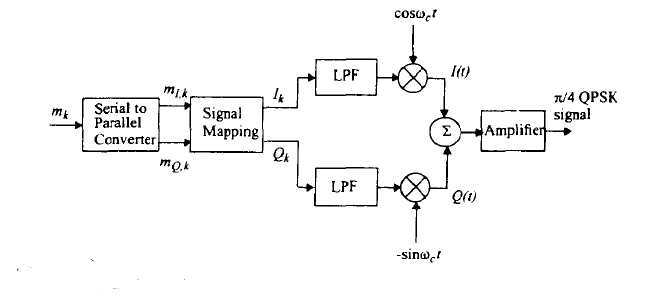
\includegraphics[width=0.6\textwidth]{dqpsk_pi_4_tx.png}
\caption{$\pi/4$-DQPSK TX}
\end{figure}

\begin{equation}
	s(t)=I(t)\cdot \cos{\omega_c\cdot t}+Q(t)\cdot(-\sin{\omega_c\cdot t})
\end{equation}

% Table generated by Excel2LaTeX from sheet 'Sheet1'
\begin{table}[htbp]
  \centering
    \begin{tabular}{ccc}
	\hline
    $m_{Ik}$ & $m_{Qk}$ & $\phi_k$ \\
    \hline
    1     & 1     & $\pi/4$ \\
    0     & 1     & $3\pi/4$ \\
    0     & 0     & $-3\pi/4$ \\
    1     & 0     & $-\pi/4$ \\
    \hline
    \end{tabular}%
  \caption{Input Bits Pair}
  \label{tab:dqpsk_pi_4}%
\end{table}

其中$I(t)$和$Q(t)$可能会取0, +1, -1, $+\frac{1}{\sqrt{2}}$, $-\frac{1}{\sqrt{2}}$

若$\theta_0=0\deg$, 输入比特流为\textbf{0, 0, 1, 0, 1, 1}, 根据表\ref{tab:dqpsk_pi_4}, 求幅值大小. 

以I为$x$轴, Q为$y$轴画单位圆. 

\begin{itemize}
	\item \textbf{0, 0}, $\theta_1=\theta_0-3\pi/4$, 对应到单位圆上的$I_1(t)$, $Q_1(t)$幅度则是$(-0.707,-0.707)$
	\item \textbf{1, 0}, $\theta_2=\theta_1-\pi/4=-\pi$, 对应到单位圆上的$I_2(t)$, $Q_2(t)$幅度则是$(-1,0)$
	\item \textbf{1, 1}, $\theta_3=\theta_2+\pi/4$, 对应到单位圆上的$I_3(t)$, $Q_3(t)$幅度则是$(-0.707,-0.707)$
\end{itemize}

可以用非相干差分检测即使缺少了相干编码. 


\subsection{RX}

\begin{figure}[H]
\centering
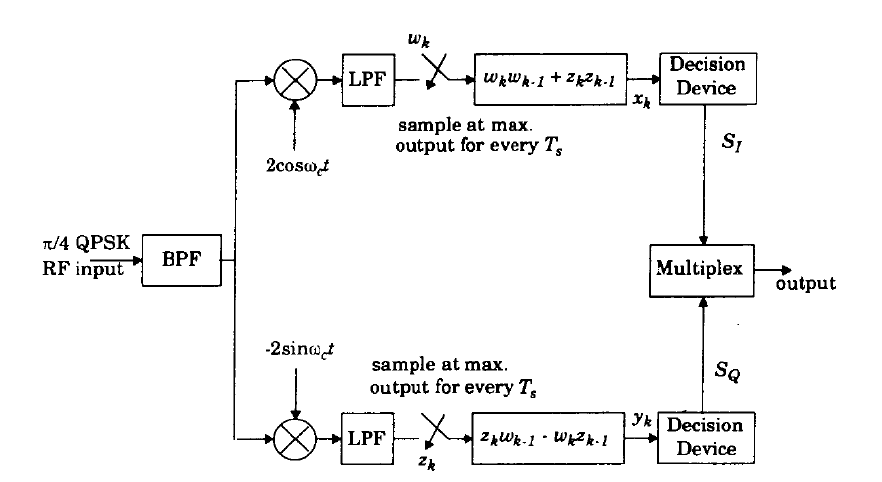
\includegraphics[width=0.6\textwidth]{qdpsk_pi_4.png}
\caption{$\pi/4$-DQPSK RX}
\end{figure}

基带差分检测, 接收得到的$I_k(t)$和$Q_k(t)$带有噪声

判决如下
\begin{align*}
	S_I=1\text{, if } x_k>0 \text{ or } S_I=0\text{, if } x_k<0 \\
	S_Q=1\text{, if } y_k>0 \text{ or } S_Q=0\text{, if } y_k<0
\end{align*}

如(-0.7,-0.7), (0.7,-0.7), (0.7, 0.7), 可以得到\textbf{0, 0, 1, 0, 1, 1}




\section{M Sequence}
最长线性移位寄存器的简称. 周期为
\begin{equation}
	P=2^n-1
\end{equation}

\subparagraph{游程} 连续0或者1的个数. 

\subparagraph{自相关系数} 有两串二进制串, 假设$A$为对应码元相同的数目, $D$为对应码元不同的数目, 则自相关系数为
\begin{equation}
	\frac{A-D}{P}=\frac{A-D}{A+D}
\end{equation}

\subparagraph{互相关函数}
\begin{equation}
	R_{xy}(\tau)=A-D
\end{equation}
\subparagraph{Gold 码} 两个m序列优选对XOR($\oplus$)

\section{Walsh–Hadamard code}
Walsh 哈达姆码, 有四个参数
\begin{itemize}
	\item 时基 (Time Base)
	\item 起始时间
	\item 振幅
	\item 列率 (Sequency)
	\subitem 频率$f$的概念在此不适用. 是Walsh的单位时间内符号变更数目的一半. 
\end{itemize}
\begin{itemize}
	\item 自相关=1
	\item 互相关=0
	\item (满足以上两点为正交码)

	\item Walsh函数是一种非正弦的完备正交函数系
	\item Walsh函数仅有可能的取值 +1和-1(或0和1)
	\item Walsh函数比较适合于用来表达和处理数字信号

	\item 哈达码矩阵可以用于产生沃尔什函数
	\item 哈达码矩阵H是由+1和-1元素构成的正交方阵
	\item 哈达码矩阵H的任意两行(或两列)都是互相正交的
	\item 哈达码矩阵H任意两行(或两列)的对应位相乘之和等于零
	\item 哈达码矩阵H任意两行(或两列)的相同位(A)和不同位(D)是相等
	\item 哈达码矩阵H的任意两行(或两列)的互相关函数为零
\end{itemize}
64阶正交Walsh码有64个两两正交的码序列. ($64\times 64$的矩阵, 任意两行都可以作为正交的码序列)

\section{OFDM}
OFDM的基本参数有
\begin{itemize}
	\item Bandwidth
	\item Bit Rate
	\item Guard Interval
\end{itemize}

\begin{itemize}
	\item 保护间隔移动环境信道的时延扩展的4倍
	\item OFDM 符号周期长度为保护间隔的6倍 (包括保护间隔)
	\item 符号周期长度为保护间隔的5倍 (不包括保护间隔)
	\item 子载波间隔为保护间隔的5倍的倒数 (频率) (不包括保护间隔)
	\item 子载波个数. 带宽需求 $N=B/\Delta f$
\end{itemize}

假定系统带宽为450 kHz, 最大多径时延为32 $\mu s$, 传输速率在 280$\sim$840 kb/s 间可变 (不要求连续可变) 求OFDM的基本参数

保护间隔
\begin{equation}
	T_{\text{Guard Interval}} =4\cdot \text{时延}= 4\times 32 \mu s= 128 \mu s 
\end{equation}
子载波间隔
\begin{equation}
	\Delta f = \frac{1}{5\cdot T_{\text{Guard Interval}}}=1.56\text{ kHz} 
\end{equation}
子载波个数(最大)
\begin{equation}
	N=\frac{B}{\Delta f}=\frac{450}{1.56}=288
\end{equation}
比特率

BPSK\footnote{$2^1=2$}可传送1个bit数据, 16QAM\footnote{$2^4=16$}可传送4个bit数据、QPSK\footnote{$2^2=4$}可传送2个bit数据; 若使用冗余编码则考虑码率. 若码率为1(不编码), 则有比特率
\begin{equation}
	R_b=\frac{N}{\underset{\text{包括保护间隔}}{T_{\text{Symbol }}}}\times \log_2{\text{NXSK}}
\end{equation}

\chapter{Radio Propagation}
 \section{Channel}
\textbf{由于移动通信环境是时变的,电波传播会引起一些特有的现象,从而影响通信系统的性能。}
\begin{itemize}
	\item 多径效应
	\item 弥散损耗 (dispersion loss) \footnote{多普勒频移?}
	\item 阴影效应 (Shadowing)
	\subitem 阴影效应是指在无线通信系统中,移动台在运动的情况下,由于大型建筑物和其他物体对电波的传输路径的阻挡而在传播接收区域上形成半盲区,从而形成电磁场阴影,这种随移动台位置的不断变化而引起的接收点场强中值的起伏变化叫做阴影效应。阴影效应是产生慢衰落的主要原因。
	\item 频带扩展
\end{itemize}

 无线信道色散现象的成因,会计算相关带宽和相关时间,掌握衰落的四种类型(平坦衰落,频率选择性, 快衰落,慢衰落)及判断标准。


 \paragraph{大尺度衰落} (路径损耗和阴影衰落属于大尺度衰落)
 \begin{itemize}
	\item 在数百米或数千米的区间内,长区间中心值随距离基站位置的变化而变化,且变化规律是接收平均功率与d的n次方成反比。
	\item 在数百米波长的区间内,信号短区间中心值缓慢变动
 \end{itemize}
 \paragraph{小尺度衰落}(多径衰落属于小尺度衰落)在数十米波长范围内,信号场强瞬时值快速变化,这是多径衰落引起的,对信号求平均值, 可以得到短区间中心值。

 \paragraph{多径衰落信道的主要参数}
 \begin{itemize}
	 \item 多径导致时延扩展 (实践色散), 时域波形展宽, 信号带宽$B_s$ 大于相干带宽$B_c$时发生频率选择性衰落 (平坦衰落要求信号带宽远小于相干带宽)
	 \item 多普勒效应导致频域扩展 (频率色散) $T_s$>$T_c$ 快衰落 (时间选择性衰落)
 \end{itemize}

 \paragraph{相干带宽} 信号在一定频率范围内(在相干带宽内)传输时, 不同频率分量遭受的衰落具有一致性
 \paragraph{相干时间} 信道冲激响应维持不变的时间间隔的统计平均值 (在一定时间间隔内, 两个到达的信号具有很强的相关性)

%  \paragraph{路径损耗接收功率比}
 \paragraph{自由空间} 与传输距离$d$和信号载频$f$有关
 \paragraph{非自由空间} 还与天线高度有关, 增加天线高度可以提高接收功率
 \paragraph{瑞利分布} 无直达径, 仅有大量反射波信号
 \paragraph{莱斯分布} 有直达径 (直达径减弱退化为瑞利分布)

 \section{陆地移动性信道的传输损耗}
 \subsection{自由空间传播模型}
 弗里斯传输方程. $L_{fs}$即free space. 
 \begin{align*}
	 \underset{\text{dB}}{L_{fs}}=32.44+20\cdot \lg {f_{\text{MHz}}}+20\cdot \lg {d_{\text{km}}}
 \end{align*}
 \subsection{中等起伏地形市区上传播损耗的中值}
 市区基本损耗中值$A_m(f,d)$, 基站天线高度增益因子$H_b(h_b,d)$, 移动台天线高度增益因子$H_m(h_m,f)$. 
 \begin{figure}[H]
 \centering
 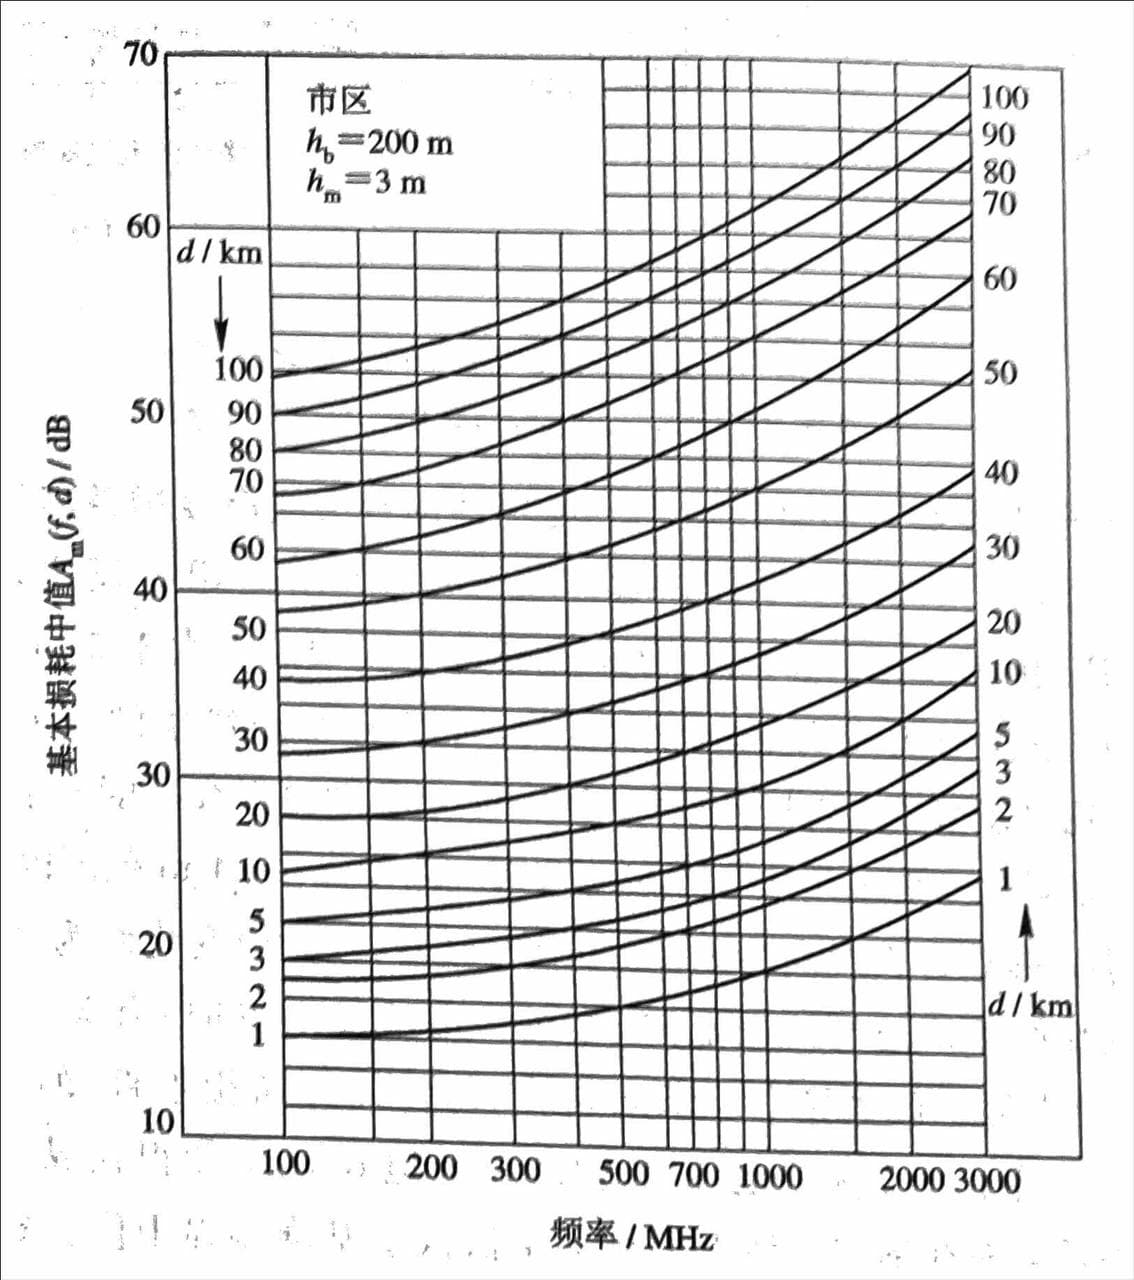
\includegraphics[width=0.33\textwidth]{A_m.jpg}
 \caption{中等起伏地上市区基本损耗中值$A_m$}
 \end{figure}
 \begin{figure}[H]
 \centering
 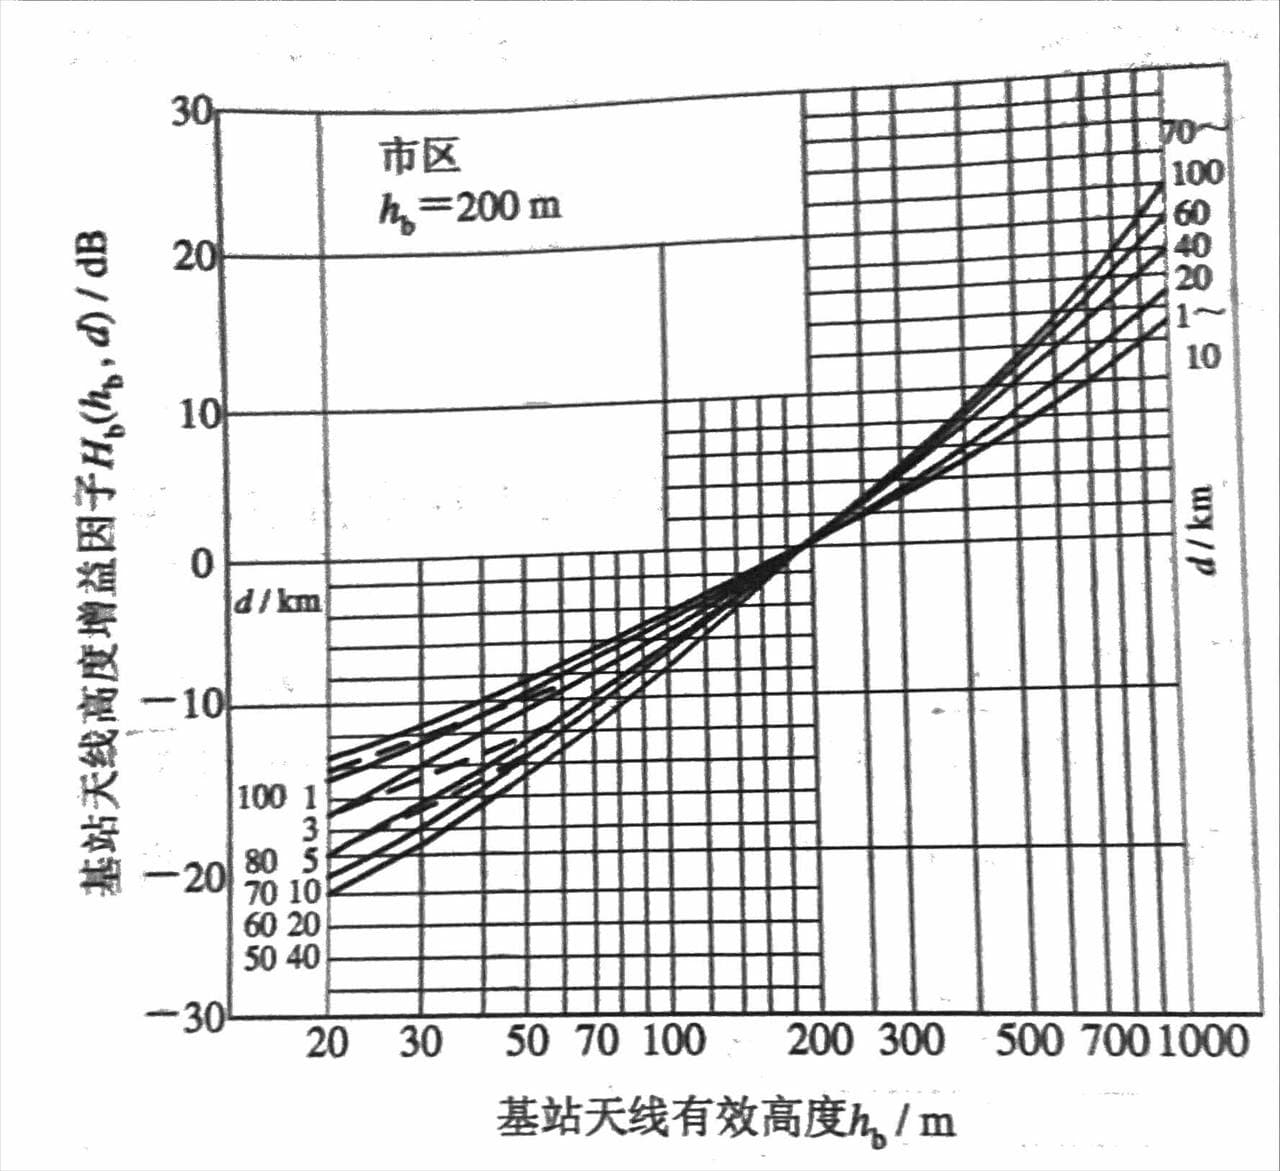
\includegraphics[width=0.33\textwidth]{H_b.jpg}
 \caption{基站天线高度增益因子$H_b$}
 \end{figure}
 \begin{figure}[H]
 \centering
 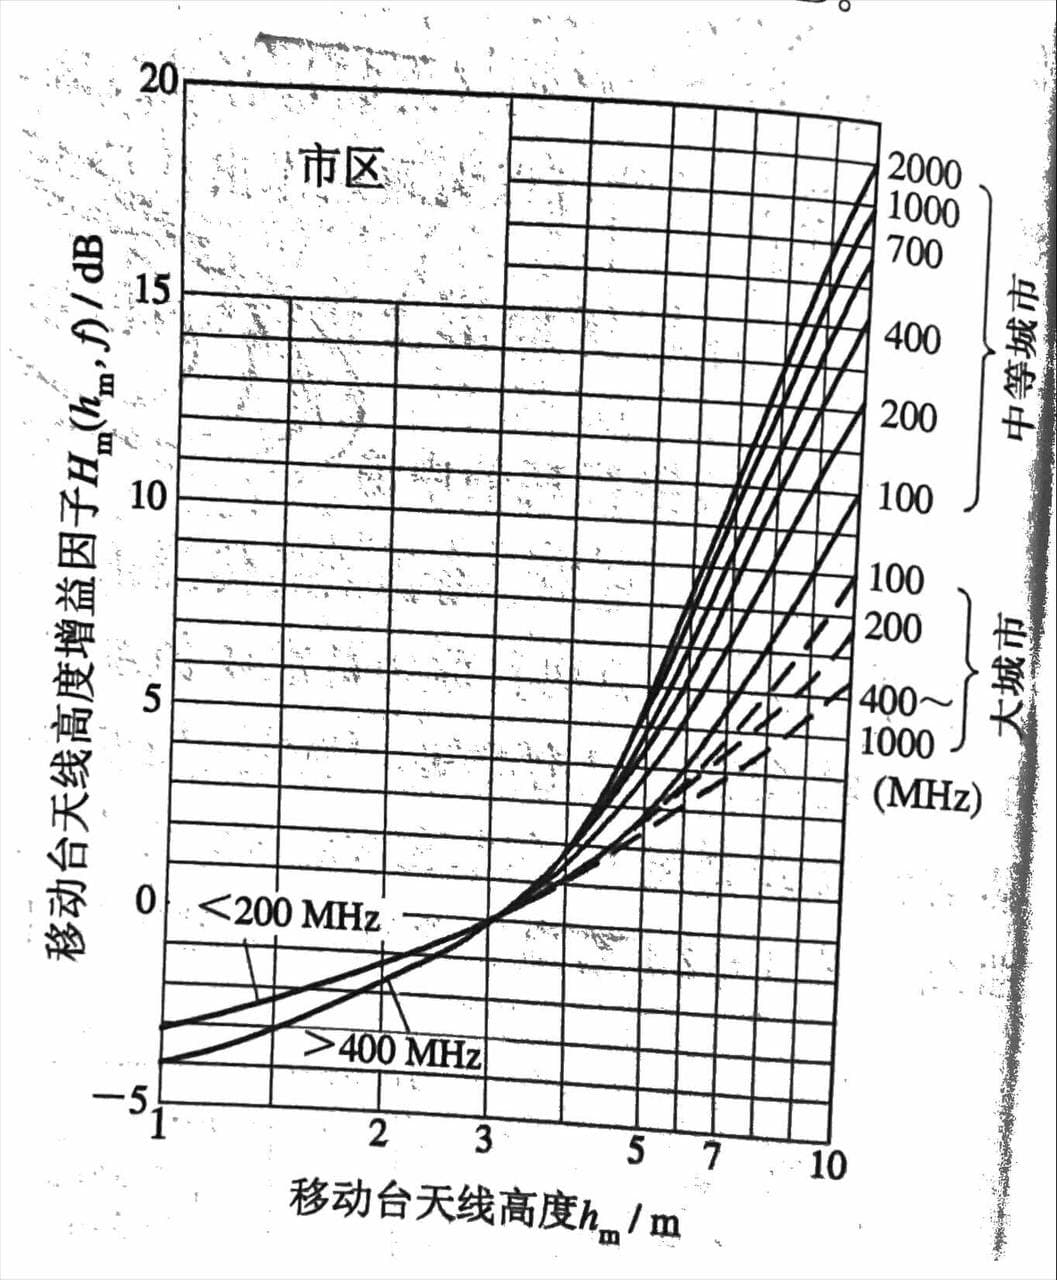
\includegraphics[width=0.33\textwidth]{H_m.jpg}
 \caption{移动台天线高度增益因子$H_m$}
 \end{figure}
可以得到传播路径损耗中值
 \begin{equation}
	 L_T=L_{fs}+A_m(f,d)-H_b(h_b,d)-H_m(h_m, f)
 \end{equation}

 基站天线高度增益因子$H_b$, 当$h_b>200m$时, $H_b>0\text{ dB}$. 反之亦然. 

 \paragraph{接收功率}假设发射功率为$P_T=10W=10\cdot \lg{10}=10\text{ dB}$, 基站天线增益6 dB, 移动台天线增益0 dB. 可以有移动台天线得到的信号功率中值. 
 \begin{align*}
	 P_P&=P_T+G_b+G_m-L_T \\
	 &=10+6+0-L_T
 \end{align*}
%  \begin{align*}
% 	 p(d)= L(d)\cdot S(d) \cdot R(d)
%  \end{align*}
%  \begin{enumerate}
% 	\item 路径损耗$L(d)$ 与d平均的$n$次方成反比,$n$为路径衰减因子,自由空间$n=2$, —般$n=3〜5$.
% 	\item 阴影衰落$S(d)$由于地形起伏、建筑物、其他障碍物对电波的遮蔽引起的衰落。
% 	\item 多径衰落$R(d)$多径传播而引起的衰落°
%  \end{enumerate}
\section{移动信道的传播模型}
 \subsection{Okumura-Hata model}
 奥村-秦模型
 \subsection{COST-231 model}
 Walfish-池上模型
 \subsection{室内(办公室)模型}


 \section{Interference}
 无线电干扰的分类及解决方法
 \subsection{同频干扰}所有落在接收机通带内的与有用信号频率相同的无用信号的干扰
\paragraph{解决方法}增加同频复用距离

\subsection{邻道干扰}指相邻信道或邻近信道的信号相互干扰。
\paragraph{解决方法}
\begin{itemize}
	\item 减小发射机带外辐射;
	\item 提高接收机的邻频道选择性;
	\item 在网络设计中,避免相邻频道在同一小区或相邻小区内使用。
\end{itemize}

\subsection{互调干扰}两个或多个信号作用在通信设备的非线性器件上,产生同有用信号频率相近的组合频率,从而对通信系统构成干扰
\paragraph{解决方法}无三阶互调的频道配置方法来避免产生互调干扰
互调干扰的判定:有用信号$\omega_s$,其它信号$\omega_1,\,\omega_2,\,\omega_3$,当
\begin{align*}
	\omega_s = 2\omega_1 - \omega_2
\end{align*}
或
\begin{align*}
	\omega_s = \omega_1+\omega_2-\omega_3
\end{align*}
时发生互调干扰


\subsection{阻塞干扰}当外界存在一个离接收机工作频率较远,但能进入接收机并作用于其前端电路的强干扰信号时,由于接收机前端电路的非线性而造成对有用信号增益降低或噪声增高,使接收机灵敏度下降的现象。

\subsection{远近效应}
同频, BS收到两个距离不同的 MS 的信号, 近端的MS功率明显大于远端MS功率. 将远端MS的有用信号淹没. (CDMA)

近端对远端的干扰, 当基站同时接收从两个距离不同的移动台发来的信号时,距基站近的移动台B到达基站的功率明显要大于距离基站远的移动台A的到达功率,若二者频率相近,则距基站近的移动台B就会造成对接收距离距基站远的移动台A的有用信号的干扰或抑制,甚至将移动台A的有用信号淹没。这种现象称为近端对远端干扰,又称为远近效应。
\paragraph{解决方法}频道间隔、移动台的自动功率控制

\section{灵敏度}
Decibel-milliwatt (dBm), 灵敏度为功率单位. 
\begin{align*}
	1 \text{ dBm}= 10\cdot\lg{10^{-3}}\text{ dB}= -30\text{ dB}
\end{align*}

某手机的灵敏度为 -110 dBm, 若接收机输入阻抗为 50 $\Omega$, 试给出以电压表示的相应灵敏度。

\begin{align*}
	-110 \text{ dBm} &= (-110-30) \text{ dB} = -140 \text{ dB}\\
	-140 \text{ dB} &= 10\cdot \lg(\frac{V^2}{R}) \\
	&= 10\cdot \lg{\frac{V^2}{50\Omega}}
\end{align*}
易得
\begin{align*}
	V=0.7071 \mu V
\end{align*}
换成 dBV\footnote{由于分贝是依据功率而定义的,因此把电压比值转化为分贝,必须采用20倍对数。dB(1 VRMS)–参考电压为1V,不考虑阻抗。SI国际单位制不允许使用分贝与后缀的组合形式如dBm, dBu, dBA,等等。但这种不遵从SI单位制的表示却广泛应用于很多场合。} 得到
\begin{equation}
	V_{\text{dB}}=20\cdot\lg{(0.7071\times 10^{-6})}=-123\text{ dBV}
\end{equation}


\chapter{Fading}
\section{Diversity}
In telecommunications, a diversity scheme refers to a method for improving the reliability of a message signal by using two or more communication channels with different characteristics. Diversity is mainly used in radio communication and is a common technique for combatting fading and co-channel interference and avoiding error bursts. 

 It is based on the fact that individual channels experience different levels of fading and interference. Multiple versions of the same signal may be transmitted and/or received and combined in the receiver. Alternatively, a redundant forward error correction code may be added and different parts of the message transmitted over different channels. Diversity techniques may exploit the multipath propagation, resulting in a diversity gain, often measured in decibels.
\begin{quotation}
	分散传输,集中处理
\end{quotation}
\begin{itemize}
	\item \textbf{Time diversity 时间分集} Multiple versions of the same signal are transmitted at different time instants. Alternatively, a redundant forward error correction code is added and the message is spread in time by means of bit-interleaving before it is transmitted. Thus, error bursts are avoided, which simplifies the error correction.
	\subitem 以超过\textbf{信道相关时间的时间间隔}重复发送信号, 以便让再次收到的信号具有独立的衰弱环境, 被广泛用于扩频 CDMA 中的 RAKE 接收机中 
	\subitem \textbf{使用} RAKE接收机, WCDMA 中的HARQ(混合自动重传) \footnote{Hybrid Automatic Repeat-reQuest}
	\item \textbf{Frequency diversity 频率分集} The signal is transmitted using several frequency channels or spread over a wide spectrum that is affected by frequency-selective fading. Later examples include:
	\subitem OFDM modulation in combination with subcarrier interleaving and forward error correction
	\subitem Spread spectrum, for example frequency hopping or DS-CDMA.
	\subitem 用若干载波同时传送同一信号, 各路载波之间的频率间隔要大于或者等于相关带宽(Coherence Bandwidth) , 在接收端对不同频率的信号进行合成. TDMA 系统中频率分级可由均衡器获得, GSM使用跳频获得频率分集. 
	\item \textbf{Space diversity 空间分集} The signal is transmitted over several different propagation paths. 
	\subitem In the case of wired transmission, this can be achieved by transmitting via multiple wires. 
	\subitem In the case of wireless transmission, it can be achieved by antenna diversity using multiple transmitter antennas (transmit diversity) and/or multiple receiving antennas (reception diversity). 
	\subitem 大规模 MIMO\footnote{Multi-input Multi-output 是一种用来描述多天线无线通信系统的抽象数学模型,能利用发射端的多个天线各自独立发送信号,同时在接收端用多个天线接收并恢复原信息。} 天线阵列, 软切换. 
	\item 极化分集
	\item 场分量分集
	\item 角度分集
\end{itemize}

\subsection{Combining}
分集合并
\subsubsection{Selection Combining}
加权系数只有一项为1, 其余为0. 进行信噪比比较, 选择其中有较高信噪比的之路接到接收机的共用部分
\begin{figure}[H]
\centering
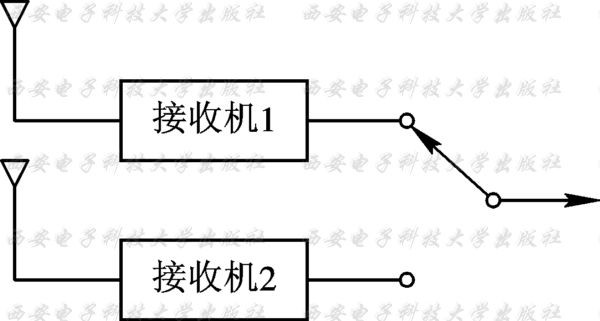
\includegraphics[width=0.5\textwidth]{sc.jpg}
\caption{SC}
\end{figure}

设第$k$支路的信号功率为$\frac{r_k^2}{2}$, 噪声功率为$N_k$, 可以得到第$k$支路的SNR为
\begin{equation}
	\gamma_k=\frac{r_k^2}{2\cdot N_k}
\end{equation}
只有全部$M$个支路的信噪比都达不到某一门限值$\gamma_t$时, 才会出现通信中断
\begin{equation}
	P_M(\gamma_S\leq\gamma_t)=\prod_{k=1}^M P_k(\gamma_k\leq\gamma_t)
\end{equation}
设$r_k$的起伏服从瑞利分布. 

\subsubsection{Equal-Gain Combining}
每一支路信号包络$r_k(t)$简写为$r_k$
\begin{figure}[H]
\centering
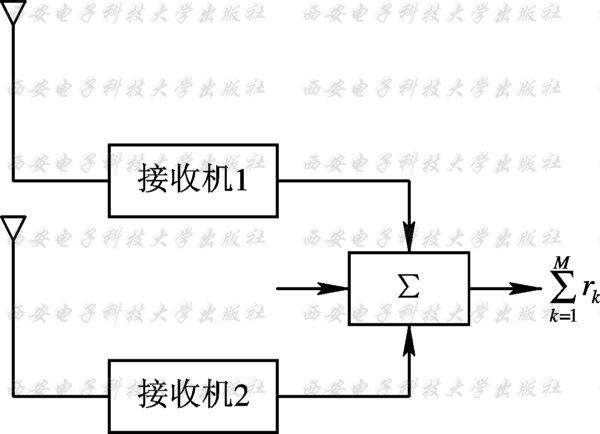
\includegraphics[width=0.5\textwidth]{egc.jpg}
\caption{EGC}
\end{figure}

\begin{align*}
	r_{\text{EGC}}=\sum_{k=1}^M r_k
\end{align*}
\subsubsection{Maximum Ratio Combining}
每一支路信号包络$r_k(t)$简写为$r_k$, 每一组路的加权系数$a_k$与信号包络$r_k$成正比, 与噪声功率$N_k$成反比
\begin{figure}[H]
\centering
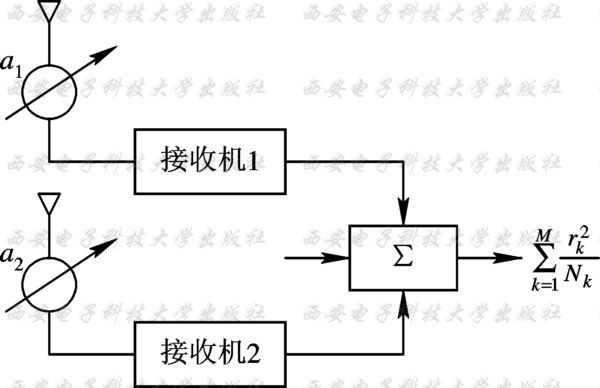
\includegraphics[width=0.5\textwidth]{mrc.jpg}
\caption{MRC}
\end{figure}

\begin{align*}
	a_k &= \frac{r_k}{N_k} \\
	r_{\text{MRC}}&=\sum_{k=1}^M \frac{r_k^2}{N_k}
\end{align*}

\section{Interleaving}
% [Burst error-correcting code - Wikipedia](https://en.wikipedia.org/wiki/Burst_error-correcting_code#Interleaved_codes)
% In telecommunication, trellis modulation (also known as trellis coded modulation, or simply TCM) is a modulation scheme that transmits information with high efficiency over band-limited channels such as telephone lines.
交织编码. 把一个较长的突发错误离散成为随机错误, 再利用纠正随机错误的信道编码技术来消除随即差错. 优点为在不附加任何开销的情况下使得数字通信系统获得时间分集, 不足是增加了传输时延. 

信道编码仅在检测和校正单个差错和不太长的差错串时才有效, 难以抗突发持续较长的深衰落和突发干扰, 使用交织可以数据经过无线信道后发生的差错串长度变短. 

Technique for making forward error correction more robust with respect to burst errors

\chapter{Networks}
\section{Multiple Access}
多址技术
\begin{itemize}
	\item 复用 Multiplexing, a method by which multiple analog or digital signals are combined into one signal over a shared medium
	\item 多址 Multiple access, allows several terminals connected to the same transmission medium to transmit over it over a shared medium.
\end{itemize}

Frequency Division Multiplexing, or FDM (频分复用), is a multiplexing technique for the physical layer that allows multiple low bandwidth signals to share the same high bandwidth frequency range. It is achieved by allocating a smaller frequency range to each signal that is using the same channel. 

FDMA (频分多址) stands for Frequency Division Multiple Access, a technology commonly used in mobile communications. It’s an access method for the data link layer, that uses the concepts of FDM to basically achieve the same goal. It is popular knowledge that FDMA is the use of FDM to enable multiple users to share the same physical channel for concurrent communication.

Frequency Reuse (频率再用) is the scheme in which allocation and reuse of channels throughout a coverage region is done. Each cellular base station is allocated a group of radio channels or Frequency sub-bands to be used within a small geographic area known as a cell. The shape of the cell is Hexagonal. The process of selecting and allocating the frequency sub-bands for all of the cellular base station within a system is called Frequency reuse or Frequency Planning.\textbf{采用频率再用技术的系统:蜂窝系统, 无绳电话系统}

In telecommunication, frequency sharing (频率共用) or channel sharing is the assignment to or use of the same radio frequency by two or more stations that are separated geographically or that use the frequency at different times. It reduces the potential for mutual interference where the assignment of different frequencies to each user is not practical or possible.\textbf{采用频率共用技术的系统: 无线寻呼系统, 集群通信}

\begin{itemize}
	\item FDMA
	\item TDMA
	\item CDMA
	\item SDMA (空分多址)
	\item 随机多址
\end{itemize}
 \section{Cluster} 
 簇(区群), 地理位置相邻, 但是不使用同一频率的小区组成一个 Cluster. 只有在不同的 Cluster 中可以频率复用. 
 \begin{itemize}
	 \item Cluster 可以邻接, 且保证各个相邻同信道小区之间的距离相等
	 \item 邻接之后的 Cluster 应该保证各个相邻同信道小区之间的距离相等
 \end{itemize}
 区群内的小区满足下列式子
 \begin{align*}
	 N = i^2 + ij + j^2
 \end{align*}
 $i,j$为正整数 ($i,j$不同时等于0, 但其中一个可以等于0) $i,j$ 无意义, 只是数而已

 \paragraph{同频率复用系数}
\begin{align*}
	\alpha = \frac{D}{r} = \sqrt{3\cdot N}
\end{align*}
$r$ 为小区的辐射半径 (即正六边形外接圆的半径\footnote{即正六边形的边长, 正六边形为六个等边三角形}), $D$ 为同信道小区中心之间的距离

系统容量与系统抗干扰性为矛盾. 

\subsection{大区制与小区制的优缺点}
\begin{itemize}
	\item 大区制
	\subitem \textbf{优点}网络结构简单,成本低
	\subitem \textbf{缺点}系统容量小,区域覆盖内盲区比较多,上下行增益差高\footnote{下行功率远大于上行, 移动台覆盖范围比基站小得多}
	\item 小区制
	\subitem \textbf{优点}系统容量大,减少覆盖区域内的盲区,降低上下行增益差
	\subitem \textbf{缺点}网络实现复杂
\end{itemize}

\paragraph{小区覆盖范围的影响因素}地球的曲率半径, 地形环境, 多径反射干扰, 基站发射功率,小区形状,地形环境,上下行增益差

\subsection{提高系统容量}
\begin{itemize}
	\item \textbf{小区分裂} 将拥塞的小区分为更小小区, 不变$N$的大小, 但是增加了 Cluster 的个数, 提高了信道的复用次数, 提高系统容量. 
	\item \textbf{小区扇区化} 通过定向天线来减少同频干扰
	\item \textbf{覆盖区域逼近}
\end{itemize}
\subsection{多信道共用技术}
多信道公用是指在网络内大量用户共享若干个 (有限的) 无线信道. 能使用户通话的阻塞概率明显下降, 同样信道数量和阻塞概率下用户数明显增加.

\section{Offered load (Erlang)} 
Offered load, carried load. 呼损率, 信道和总话务量的关系. 
\begin{align*}
	A &= S \cdot \lambda \\
	E & = \lambda \cdot h
\end{align*}
单位时间(一小时)内平均发生的呼叫次数$\lambda$ 的单位是次/小时, 每次呼叫平均占用信道时间(含通话时间)$S$ ($h$) 的单位是小时/次

如全网平均每小时发生20次呼叫, 平均每次呼叫的「通话时间」为三分钟, 则有
\begin{align*}
	\lambda&=20 \text{ 次/hour} \\
	S &= 3 \text{ min/次} = \frac{3}{60} \text{ hour/次} \\
	A &= \lambda \cdot S = 20 \cdot \frac{3}{60} = 1 \text{ Erlang}
\end{align*}
设单位时间内成功呼叫的次数为$\lambda_0$ ($\lambda_0<\lambda$) 则有呼损率 (blocking probability)
\begin{align*}
	B &= \frac{A-A_0}{A} \\
	&=\frac{\lambda-\lambda_0}{\lambda}
\end{align*}
\subsection{Erlang B formula} 
\begin{align*}
	B = \frac{\frac{A^n}{n!}}{\sum_{i=1}^n\frac{A^i}{i!}}
\end{align*}
因为计算过于繁杂, 通常使用表格 \ref{tab:erlang_b} , 已知呼损率$B$和信道数$n$, 可以查表得到总话务量$A$和信道利用率$\eta$
% Table generated by Excel2LaTeX from sheet 'Sheet1'
\begin{table}[htbp]
  \centering
    \begin{tabular}{ccccccc}
	\hline
    \diagbox{$n$}{$A$}{$B$} & 0.01  & 0.02  & 0.03  & 0.04  & 0.05  & 0.1 \\
    \hline
    1     & 0.01  & 0.02  & 0.031 & 0.042 & 0.053 & 0.111 \\
    2     & 0.153 & 0.223 & 0.281 & 0.333 & 0.381 & 0.595 \\
    3     & 0.455 & 0.602 & 0.715 & 0.812 & 0.899 & 1.271 \\
    4     & 0.869 & 1.092 & 1.259 & 1.399 & 1.524 & 2.045 \\
    5     & 1.36  & 1.657 & 1.875 & 2.057 & 2.218 & 2.881 \\
    6     & 1.909 & 2.276 & 2.543 & 2.764 & 2.96  & 3.757 \\
    7     & 2.501 & 2.935 & 3.25  & 3.509 & 3.738 & 4.666 \\
    8     & 3.127 & 3.627 & 3.986 & 4.282 & 4.542 & 5.596 \\
    9     & 3.782 & 4.344 & 4.747 & 5.079 & 5.37  & 6.546 \\
    10    & 4.46  & 5.083 & 5.529 & 5.895 & 6.215 & 7.51 \\
    11    & 5.16  & 5.841 & 6.327 & 6.726 & 7.075 & 8.486 \\
    12    & 5.875 & 6.614 & 7.14  & 7.572 & 7.95  & 9.472 \\
    13    & 6.606 & 7.401 & 7.966 & 8.43  & 8.834 & 10.467 \\
    14    & 7.351 & 8.2   & 8.803 & 9.297 & 9.728 & 11.471 \\
    15    & 8.108 & 9.009 & 9.65  & 10.173 & 10.631 & 12.482 \\
    16    & 8.875 & 9.828 & 10.504 & 11.059 & 11.543 & 13.5 \\
    17    & 9.651 & 10.655 & 11.368 & 11.951 & 12.459 & 14.518 \\
    18    & 10.436 & 11.49 & 12.237 & 12.85 & 13.384 & 15.548 \\
    19    & 11.229 & 12.332 & 13.114 & 13.754 & 14.313 & 16.579 \\
    20    & 12.03 & 13.181 & 13.997 & 14.663 & 15.249 & 17.612 \\
    21    & 12.837 & 14.035 & 14.884 & 15.578 & 16.186 & 18.649 \\
    22    & 13.651 & 14.894 & 15.778 & 16.5  & 17.131 & 19.69 \\
    23    & 14.469 & 15.759 & 16.674 & 17.424 & 18.078 & 20.734 \\
    24    & 15.294 & 16.629 & 17.575 & 18.352 & 19.028 & 21.779 \\
    25    & 16.124 & 17.503 & 18.481 & 19.284 & 19.983 & 22.83 \\
    26    & 16.958 & 18.381 & 19.392 & 20.217 & 20.941 & 23.88 \\
    27    & 17.796 & 19.265 & 20.303 & 21.156 & 21.901 & 24.937 \\
    28    & 18.64 & 20.149 & 21.219 & 22.097 & 22.866 & 25.99 \\
    29    & 19.486 & 21.038 & 22.139 & 23.042 & 23.832 & 27.049 \\
    30    & 20.336 & 21.931 & 23.06 & 23.987 & 24.8  & 28.11 \\
    \hline
    \end{tabular}%
  \caption{Erlang B Table}
  \label{tab:erlang_b}%
\end{table}%


\paragraph{信道利用率} 对于多信道共用的移动通讯网
\begin{align*}
	\eta = \frac{A_0}{n}=\frac{A\cdot (1-B)}{n}
\end{align*}
$A_0$为完成话务量, $n$为共用信道数. 


\paragraph{忙时话务量} 最忙一小时内的话务量与全天话务量之比称为集中系数$k$, 一般$k=10\%\sim 15\%$.
设每个用户每天打$C$次电话\footnote{$C$的单位为「次/天」}, 每次通话$T$秒\footnote{$T$的单位为「秒/次」}, 则每个用户的忙时话务量$a$为
\begin{align*}
	a = C\cdot T\cdot k\cdot \frac{1}{3600}
\end{align*}
一般按照$a = 0.02\sim 0.03$设计系统

$n$为共用信道数, 每个信道所能容纳的用户数$m$, 全网的用户数(系统所容纳的用户数)为
\begin{align*}
	M = m\cdot n
\end{align*}
\begin{align*}
	m=\frac{A/n}{a}=\frac{\frac{A}{n}\cdot 3600}{C\cdot T\cdot k}
\end{align*}
\chapter{TDMA}
\section{GSM}
\subsection{Frequency} 
\label{sec:gsm:frequency}
\begin{itemize}
	\item 890MHz$\sim$ 960MHz 工作频段
	\item 890 $\sim$ 915MHz (25MHz) Uplink (MS$\rightarrow$BS)\footnote{低频需要的功率较小}
	\item 915 $\sim$ 935MHz (20MHz) 保护频段
	\item 935 $\sim$ 960MHz (25MHz) Downlink  (BS$\rightarrow$MS)
	\item 200KHz 信道(载频) 间隔
\end{itemize}
\begin{align*}
	f_l(n)&=(890+0.2\cdot n) \text{MHz} \\
	f_h(n)&=(935+0.2\cdot n) \text{MHz}
\end{align*}
其中载频编号为$n=1\sim 124$

\subsection{Mobile Station}
在GSM中,一个移动台由四个主要部分组成
\begin{itemize}
	\item 移动终端(Mobile Termination,简称MT),它提供一些公共的功能,例如:无线电信号传输和切换, 语音编解码, 错误检测与纠正,信令交互和访问SIM卡。 设备串号(IMEI)是关联到移动终端(MT)的。 它是综合业务数字网(ISDN)接入中的网络终端是等价的。
	\item 终端设备 (Terminal Equipment,简称TE)是指任何连接到移动台、并向用户提供服务的设备。 它并不包含任何GSM所特有的功能。
	\item 终端适配器 (Terminal Adapter)提供对移动终端(MT)的访问,就和ISDN网络终端一样,包含扩展的能力。 终端设备(TE)和移动终端(MT)通过终端适配器(TA)所进行的通信,是使用AT指令集来进行的.
	\item 用户身份模块(Subscriber Identity Module)是一个可拆卸的用户识别令牌,它储存国际移动用户识别码(IMSI),这是一个唯一的秘钥,会被共享给移动网络运营商。
\end{itemize}
在一部移动电话中,移动终端(MT)、终端适配器(TA)和终端设备(TE)是被封装在一个盒子里的,但是移动终端(MT)和终端设备(TE)功能通常是由截然不同的处理器来承担的。应用处理器完成终端设备(TE)的功能,而基带处理器完成移动终端(MT)的功能,二者之间的通信都通过一个使用AT指令集的总线来进行,而这个总线就完成终端适配器(TA)的功能。
\subsection{Base Station Subsystem}
基站子系统(Base Station Subsystem,简称:BSS)

\begin{figure}[H]
\centering
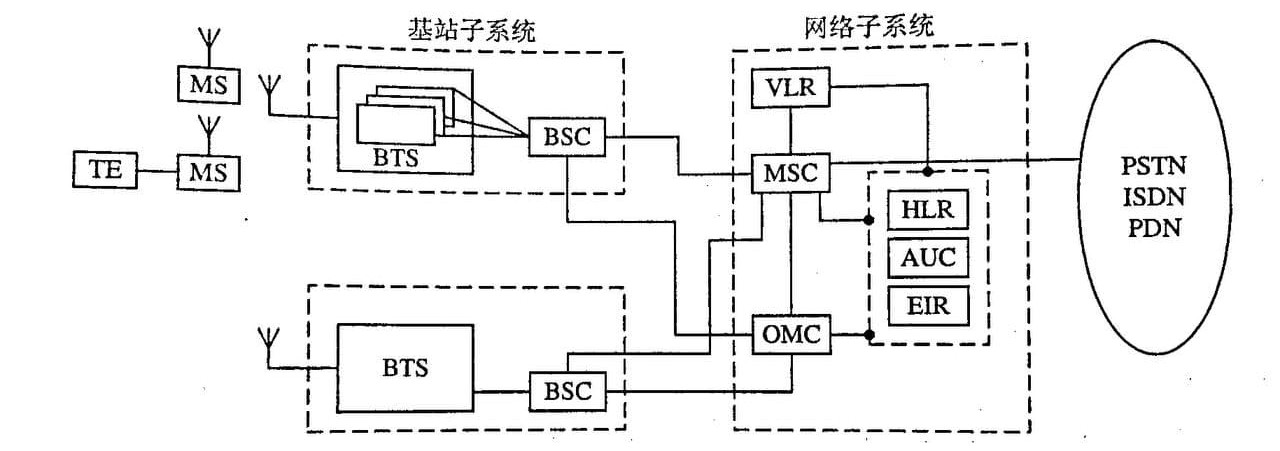
\includegraphics[width=0.8\textwidth]{gsm.jpg}
\caption{GSM}
\end{figure}
\begin{figure}[H]
\centering
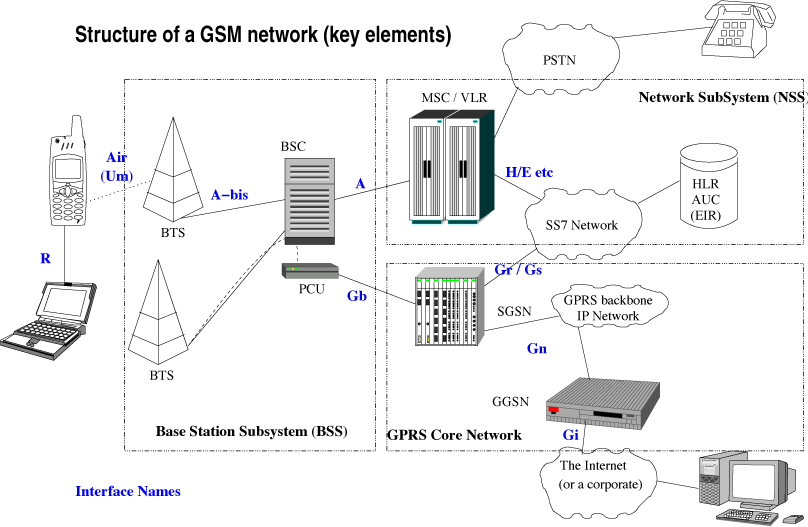
\includegraphics[width=0.8\textwidth]{Gsm_network.png}
\caption{GSM and GPRS}
\end{figure}
\begin{figure}[H]
\centering
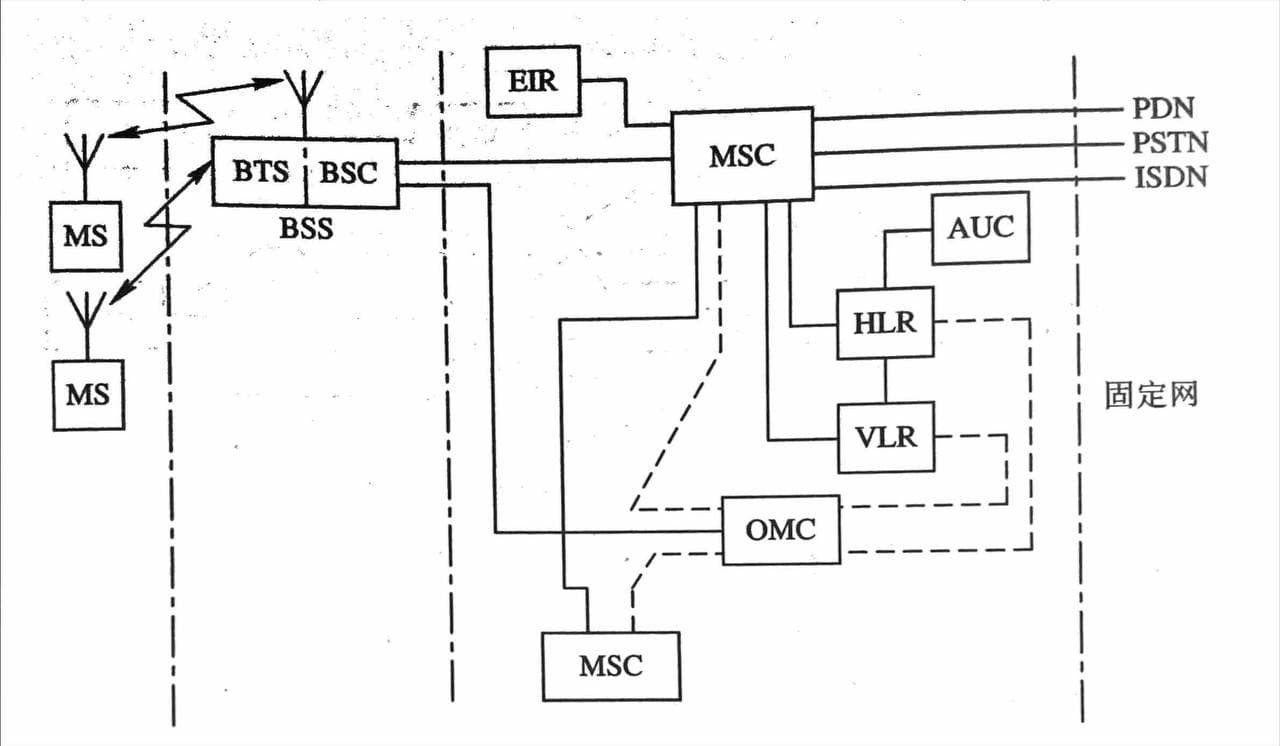
\includegraphics[width=0.8\textwidth]{cell.jpg}
\caption{数字蜂窝通信的网络结构}
\end{figure}

\subsubsection{Base Transceiver Station}
基地收发机站(Base Transceiver Station,简称:BTS)包含用于传输和接收无线电信号的设备(收发机)、天线,以及用于加密和解密与基站控制器(Base Station Controller,简称:BSC)之间的通信。
\subsubsection{Base Station Controller}
基站控制器(Base Station Controller,简称:BSC)经常被用于提供在BTS之后的智能部分。
 \subsection{Network Switching Subsystem}
 网络交换子系统(Network Switching Subsystem,简称:NSS)又称GSM核心网(GSM Core Network),是GSM系统的一个组件,它为基站网络上的移动电话漫游(mobile phones roaming)实现电话交换(call switching)和移动性管理(mobility management)功能。
 \subsubsection{Mobile Switching Center}
 \label{sec:msc}
 MSC建立(set up)和拆除(release)端到端连接,在呼叫过程中,处理可移动性(mobility)和切换(hand-over)需求,并处理计费和实时预付费账户监视。
 \begin{itemize}
	 \item 根据来自VLR的信息,当呼叫到达时,将其投送给签约用户
	 \item 将出向呼叫(outgoing calls)连接到其它的移动签约用户或PSTN
	 \item 将来自签约用户的短信投送到短信中心,反之亦然。
	 \item 安排从一个BSC到另一个BSC的切换。
	 \item 实现从一个MSC到另一个MSC的切换。
	 \item 支持补充业务(supplementary services),例如电话会议和呼叫保持。
	 \item 生成计费信息。
 \end{itemize}

 网络核心, 提供交换功能, 并面向其他功能实体, 可以从 HLR, VLR中获取用户位置登记和呼叫请求, 支持位置更新, 越区切换, 漫游等
 \subsubsection{Home Location Register}
 归属位置寄存器(Home Location Register,简称:HLR),用于获取关于该SIM卡和MSISDN(即电话号码)的数据。

 储存静态数据, 如移动用户码, 访问能力, 用户类别, 业务等, 还暂存移动用户漫游时有关动态信息数据. 
 \subsubsection{Visitor Location Register}
 拜访位置寄存器(Visitor Location Register,简称:VLR),当签约用户用户位于其归属网络之外时,提供签约用户的信息。

 从漫游移动用户的HLR中获取暂存, 动态用户的数据库
 \subsubsection{Equipment Identity Register}
 设备身份寄存器(Equipment Identity Register,简称:EIR)是一个数据库,存储关于移动设备的身份相关的讯息,以防止来自被盗的、未授权的或有缺陷的移动台的呼叫。

 存储 IMEI, 检查移动设备 (而非SIM卡) 是否被允许
 \subsubsection{Authentication Center}
 鉴权中心(Authentication Center,简称:AuC)是一个对各个对GSM核心网的连接的尝试(通常是在电话开机的时候进行)的SIM卡进行鉴权的功能。
\subsection{Interface}
只要遵守接口规范, 无论哪一家厂商生产的设备都可以用来组网, 而不必限制这些设备在开发和生产中采用何种技术. 
\begin{figure}[H]
\centering
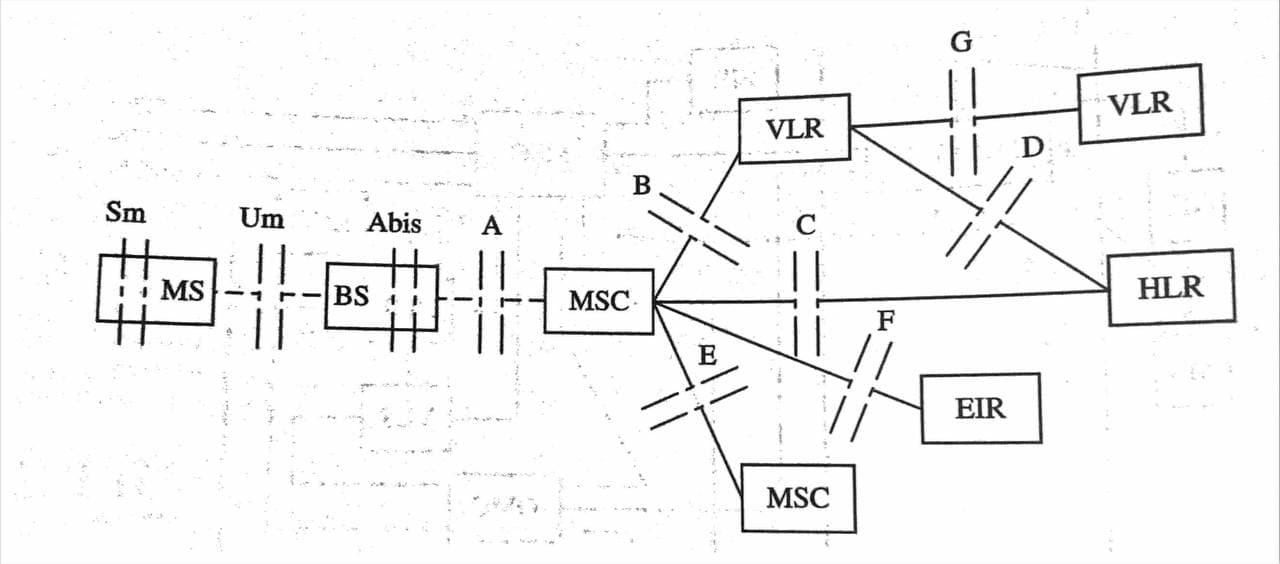
\includegraphics[width=0.8\textwidth]{cell_interface.jpg}
\caption{蜂窝系统所用的接口}
\end{figure}
\begin{figure}[H]
\centering
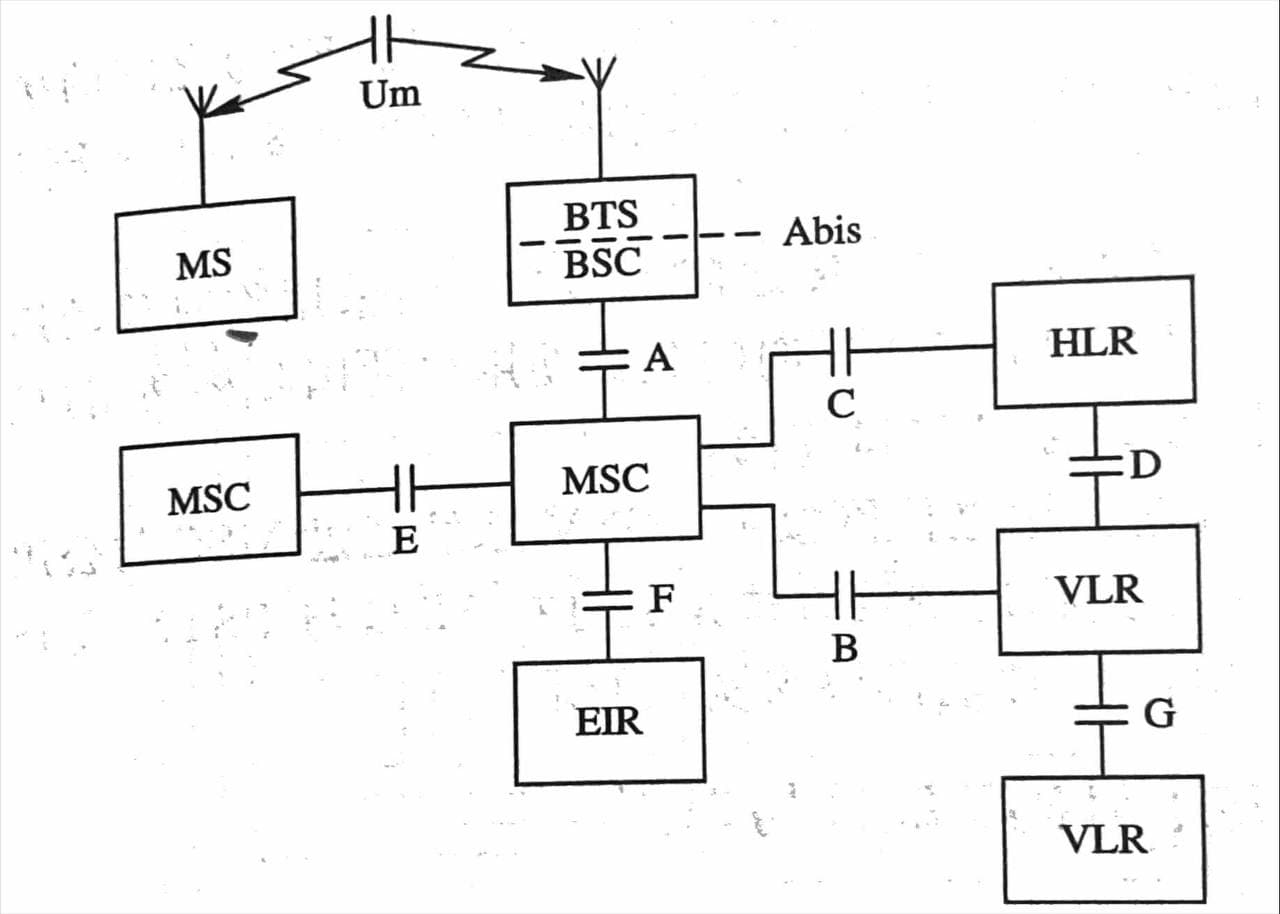
\includegraphics[width=0.8\textwidth]{gsm_interface.jpg}
\caption{GSM 接口}
\end{figure}
\begin{itemize}
	\item Sm 用户和网络之间接口, 人机接口
	\item Um 是 BS 与 MS 之间接口, 也成未无线接口或空中接口
	\item A 是 BS 和 MSC 之间接口
	\item Abis 是 BTS 和 BSC 之间接口
\end{itemize}
其余略, 使用 OSI 中的最底下三层
\begin{itemize}
	\item 网络层
	\subitem 连接管理 (CM)
	\subitem 移动管理 (MM)
	\subitem 移动资源管理 (RRM)
	\item 数据链路层
	\item 物理层
\end{itemize}
\subsubsection{Um interface}
空中接口, (MS-BS接口) The Um interface is the air interface for the GSM mobile telephone standard. It is the interface between the mobile station (MS) and the Base transceiver station (BTS).

 It is called Um because it is the mobile analog to the U interface\footnote{The U interface or U reference point is a Basic Rate Interface (BRI) in the local loop of an Integrated Services Digital Network (ISDN)} of ISDN\footnote{Integrated Services Digital Network (ISDN) is a set of communication standards for simultaneous digital transmission of voice, video, data, and other network services over the digitalised circuits of the public switched telephone network.}. 

 \subsection{Frame} 
 \label{sec:gsm:frame}
\begin{figure}
\centering
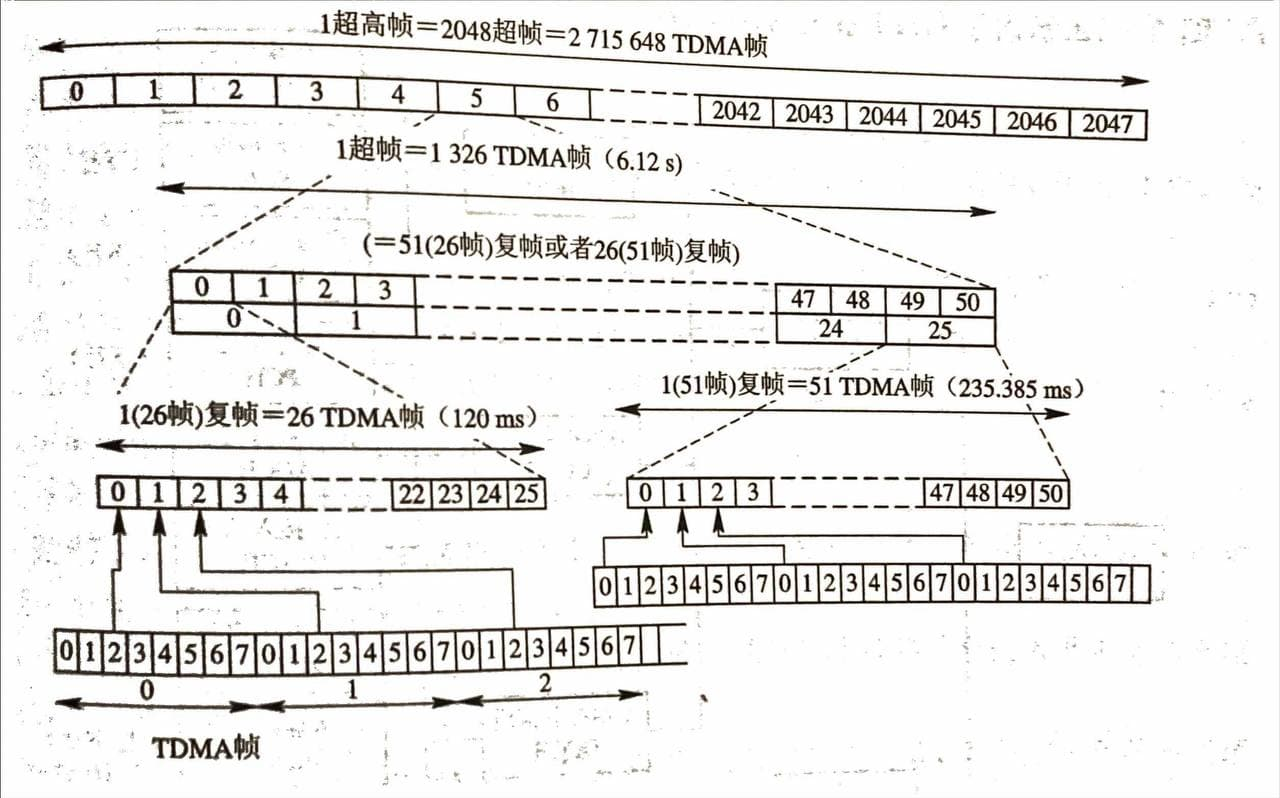
\includegraphics[width=0.8\textwidth]{gsm_frame.jpg}
\caption{GSM帧}
\end{figure}
时隙是基本的通信单位, TDMA 帧长 4.615 ms, 一个帧包含八个时隙\footnote{timeslots}, 每个时隙的长度为 0.577ms\footnote{$4.615\div 8$}. 
\begin{quotation}
	 These eight radio timeslots (or burst periods) are grouped into a TDMA frame. Half-rate channels use alternate frames in the same timeslot. The channel data rate for all 8 channels is 270.833 kbit/s, and the frame duration is 4.615 ms.
\end{quotation}
\begin{itemize}
	\item 一个超高帧 = 2048个超帧
	\item 一个超帧 = 51个复帧(业务讯息)或者26个复帧(控制讯息)
	\item 一个复帧 = 26个TDMA帧(业务讯息)或者51个TDMA帧(控制讯息)
	\item 一个TDMA = 8个时隙
\end{itemize}

上行帧退后了三个时隙, 为了便于MS调整频点便于同步. (允许移动台在这3个时隙的时间内进行帧调整以及对收发信机进行调谐和转换)

一个TDMA帧有8个时隙,其中1-7号时隙用来承载业务,0号时隙主要用来广播系统消息,所以也被称为BCCH(广播控制信道)时隙。1-7号时隙完全一样,没有区别,但是0号时隙另有玄机!

\subsection{Channel}
\begin{figure}[H]
\centering
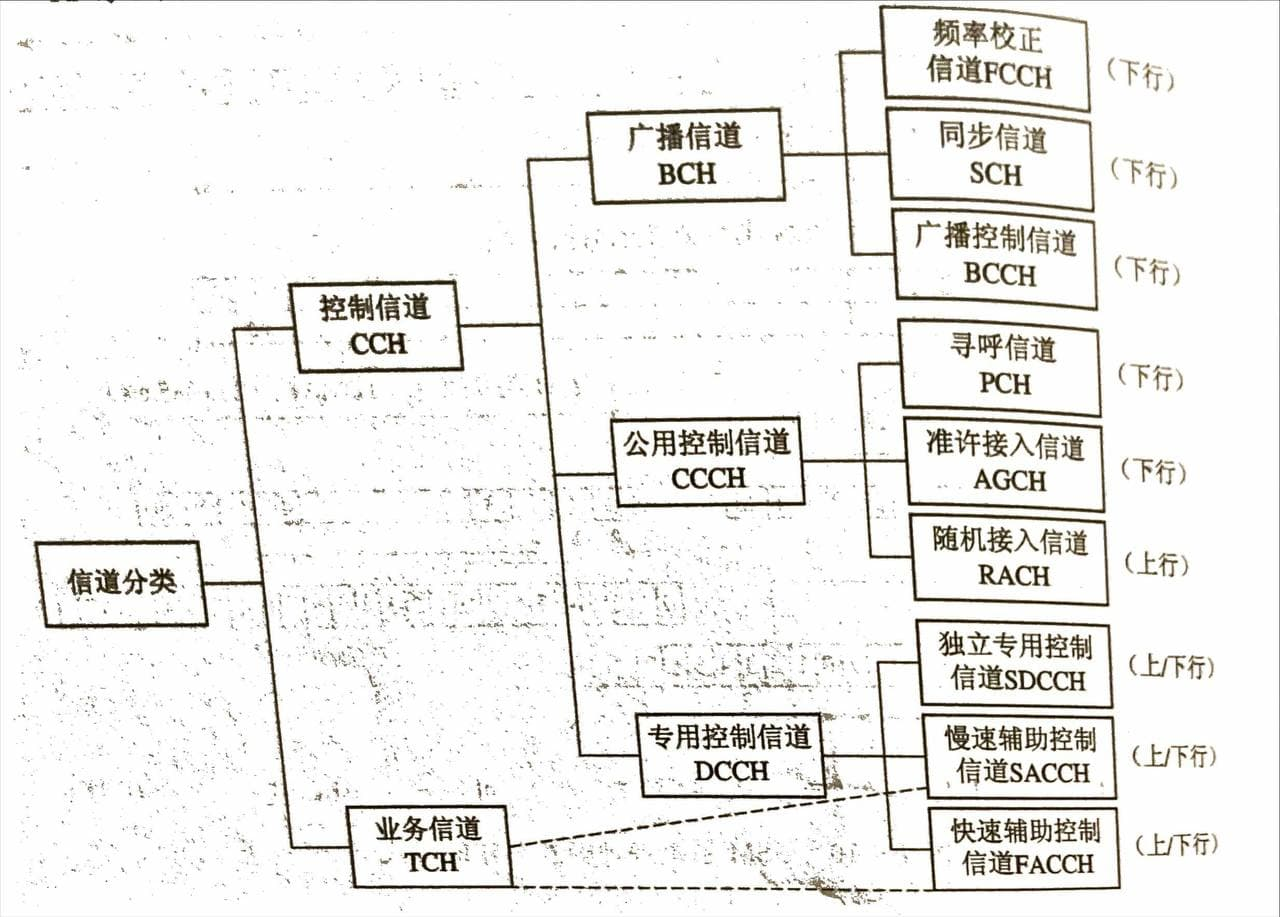
\includegraphics[width=0.7\textwidth]{gsm_chann.jpg}
\caption{GSM信道}
\begin{itemize}
	\item BCCH(Broadcast Control Channel)
	\item FCCH(Frequency Correction Channel)
	\item SCH(Synchronization Channel)
	\item RACH(Random Access Channel)
	\item PCH(Paging Channel) 寻呼信道
	\item CCCH(Common Control Channel)
	\item FACCH(Fast Associated Control Channel)
	\item SACCH(Slow Associated Control Channel)
	\item SDCCH(Standalone Dedicated Control Channel)
	\item TCH(Traffic Channel)
	\item AGCH(Access Grant Channel)
\end{itemize}
基站识别码在SCH, 位置区识别码BCCH, 测量基站信号强度SACCH

\end{figure}
\subparagraph{主叫} RACH$\rightarrow$AGCH$\rightarrow$SDCCH$\rightarrow$TCH
\subparagraph{被叫} PCH$\rightarrow$RACH$\rightarrow$AGCH$\rightarrow$SDCCH$\rightarrow$TCH

MS在RACH上向BS发出信道请求信息, 如果BS接收成功就给这个MS分配一个专用的控制信道, 即在AGCH上向MS发送立即分配指令 (礼貌性回复), 利用DCCH\footnote{专用控制信道}与BS建立信令链路, 经过BS向MSC发送业务请求, VLR鉴权后给MS分配一个TMSI, MS向MSC建立呼叫请求, BS如果有空闲的TCH\footnote{业务信道}

\subsection{Burst}
\begin{itemize}
	\item Normal Burst 常规突发脉冲序列 用于业务信道和专用的控制信道(上下行)
	\item Frequency Correction Burst 频率矫正同法脉冲序列. 用于矫正移动台的载波频率 (下行)
	\item Synchronization Burst 同步突发脉冲序列, 用于移动台的时间同步(下行)
	\item Access Burst 用于MS向BS提出入网申请 (上行, 在RACH上传送)
\end{itemize}

\subsection{SS}
每个TDMA帧 4.615ms 跳频一次, 每秒跳217次\footnote{1s/4.615ms}. 属于慢调频, 因为不实现扩频. 通过跳频躲避干扰提高抗干扰性能. 

\subsection{* Authentication}
\begin{figure}[H]
\centering
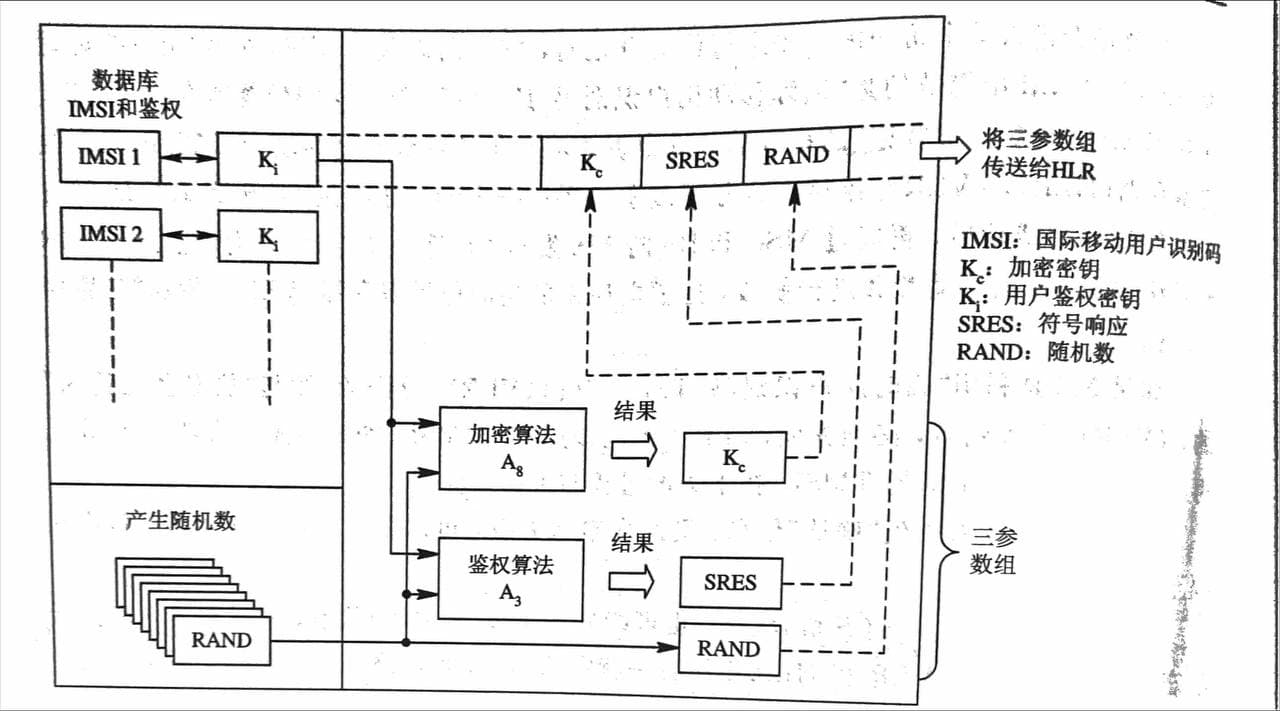
\includegraphics[width=0.7\textwidth]{gsm_auc.jpg}
\caption{AUC}
\end{figure}

\begin{figure}[H]
\centering
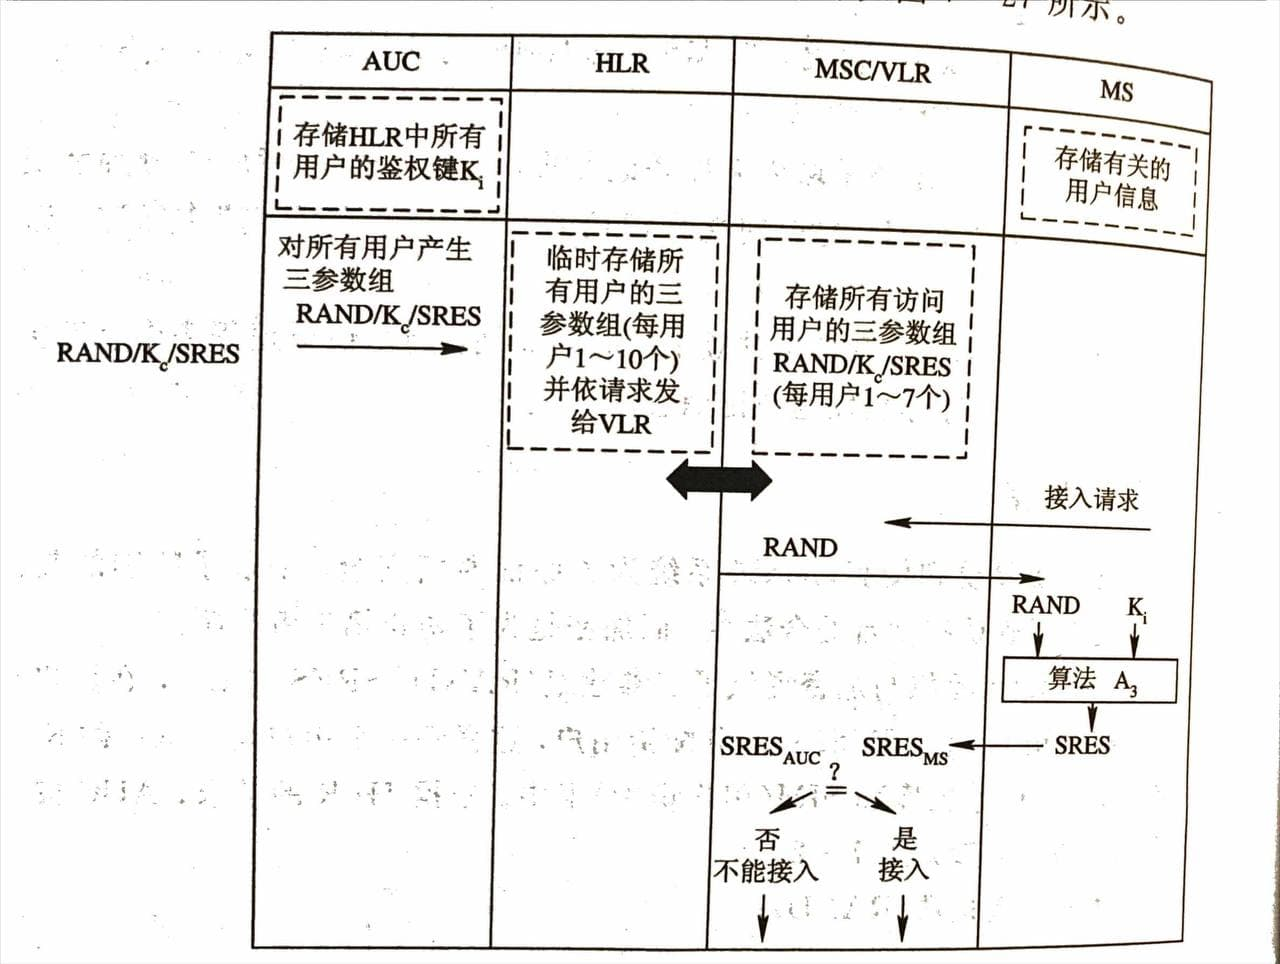
\includegraphics[width=0.7\textwidth]{gsm_auc_flow.jpg}
\caption{鉴权程序}
\end{figure}

三参数组: RAND, SRES和$K_c$. 

入网时, 用户鉴权密钥$K_i$连同 IMSI 一起分配给用户, 每个用户均有唯一的 $K_i$ 和 ISMI. 它们存储于AUC和SIM卡中. 根据HLR请求, AUC按下列步骤产生三参数
\begin{itemize}
	\item 产生RAND
	\item 通过加密算法$A_8$, 输入$K_i$和RAND算出密钥$K_c$
	\item 通过鉴权算法$A_3$, 输入$K_i$和RAND, 产生符号响应 (Signed Response) SRES
	\item RAND, SRES, $K_c$作为三参数组一起送给HLR
\end{itemize}
本质是验证MS和BS的鉴权键$K_i$是否相同, 但$K_i$怕被截获, 故MS用RAND和自己的$K_i$输入, $A_3$鉴权算法产生SRES, 在BS中的MSC处比较来自AUC的SRES和MS的SRES是否相同. 

\subsection{Identities}
\subsubsection{IMSI}
国际移动用户识别码(英语:IMSI,International Mobile Subscriber Identity),是用于区分蜂窝网络中不同用户的、在所有蜂窝网络中不重复的识别码。手机将IMSI存储于一个64比特的字段\footnote{储存在SIM卡中,可用于区别移动用户的有效信息。其总长度不超过15位}发送给网络。IMSI可以用来在归属位置寄存器(HLR,Home Location Register)或拜访位置寄存器(VLR,Visitor Location Register)中查询用户的信息。为了避免被监听者识别并追踪特定的用户,大部分情形下手机和网络之间的通信会使用随机产生的临时移动用户识别码(TMSI,Temporary Mobile Subscriber Identity)代替IMSI。
\subsubsection{TMSI}
Temporary Mobile Subscriber Identity

为了防止非法监听进而盗用IMSI, 当在无线链路上需要传送IMSI时, 均使用TMSI代替IMSI, 仅在位置更新失败或者MS得不到TMSI时才使用IMSI. 
\subsubsection{IMEI}
International Mobile Equipment Identity. EIR存储所有被列入黑/灰名单的设备. 

\begin{itemize}
	\item 黑名单: 禁止使用的移动设备
	\item 白名单: 合法的移动设备识别号
	\item 灰名单: 是否允许使用由运营者决定
\end{itemize}
\subsection{软硬切换}
\paragraph{软切换} 既维持旧的连接, 又同时建立新的连接, 并利用新旧连接链路的分集合并改善通信质量
\paragraph{硬切换} 在新的连接建立以前先中断旧的连接
GSM 只能采用硬切换, 因为相邻基站不同频率; IS-95 可以采用软切换, 因为相邻基站可以同频
\subsection{* GPRS}
\textbf{GPRS系统在GSM系统的基础上增加了哪些功能单元?}
增加了SGSN\footnote{Serving GPRS support node} (GPRS服务支持节点)和GGSN\footnote{Gateway GPRS support node} (GPRS网关支持节点)。



TDMA 对越区切换十分友好, GSM一帧8个时隙最多工作2个, 其余6个对周围BS的BCCH进行信号强度测量, 并用SACCH不断报告与正在服务基站周边基站的信号强度. 
\section{GSM, D-AMPS and PDC}
三种TDMA的比较. 为了统一比较各系统的容量, 设总频段W=25 MHz, 小区半径r=1 km, 每小区分三个扇区, 呼损率B=2\%,并令模拟系统的容量为 1(归一化)
\begin{figure}[H]
\centering
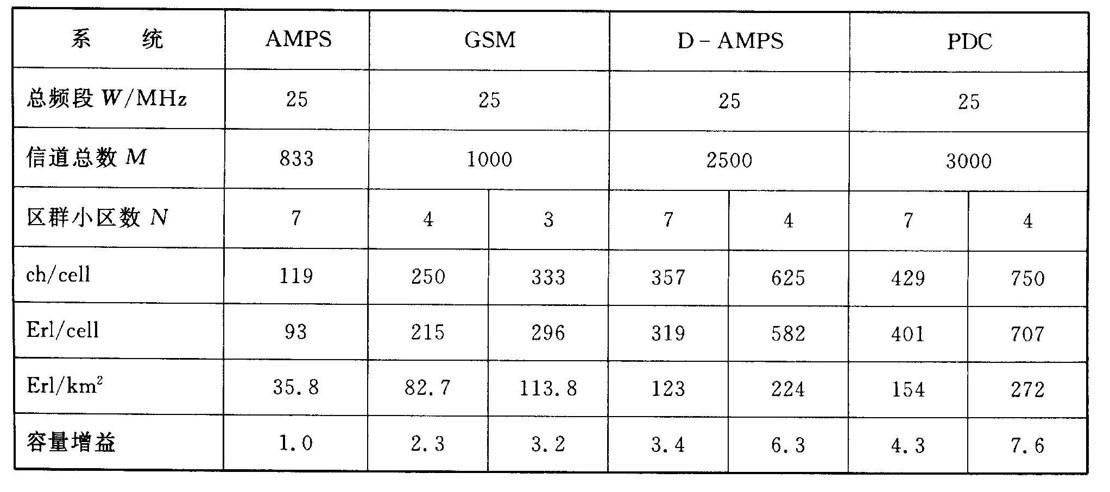
\includegraphics[width=0.7\textwidth]{tdma_cap.jpg}
\caption{三种TDMA蜂窝系统与模拟蜂窝系统的容量比较}
\end{figure}
\subsection{AMPS}
信道总数(用户总数), 易知AMPS的频带间隔为$30$ kHz. 假设区群小区数量为8. 

\begin{align*}
	M&=\frac{B_t}{\underset{\text{频道宽度}}{\Delta f}}\\
	m_c&=\frac{B_t}{\underset{\text{频道宽度/频带间隔}}{\Delta f}\times \text{小区数量}} \\
	&=\frac{25\times 10^6}{30\times 10^3\times 8}\\
	&= 119 \text{ channel/小区}
\end{align*}

可以根据$m_c$逆推得到每扇区信道数量\footnote{每个小区分为三个扇区}

\begin{equation}
	n=m_c/3\approx 40
\end{equation}

根据$n=40$, B=2\%可以查表\ref{tab:erlang_b}得到$A_0=31$ Erlang/扇区. 

每小区的话务量\footnote{每个小区分为三个扇区}$A=3\cdot A_0=93$. 

小区半径$r=1$ km, 若按正六边形计算$S=\frac{3\sqrt{3}}{2}\cdot r\approx 2.6$ $km^2$

可以得到每平方公里的话务量为

\begin{equation}
	\frac{93}{2.6}=35.8 \text{ Erlang/$km^2$}
\end{equation}
\subsection{GSM}
见\ref{sec:gsm:frequency}易知GSM的频带间隔为$200$ kHz, 见\ref{sec:gsm:frame}知时隙为8, 假设区群小区数量为4
\begin{align*}
	m_c&=\frac{B_t\times \text{Timeslot(时隙)}}{\underset{\text{频道宽度/频带间隔}}{\Delta f}\times \text{小区数量}} \\
	&=\frac{25\times 10^6\times 8}{200\times 10^3\times 4}\\
	&= 250 \text{ channel/小区}
\end{align*}

若每个小区分为三个扇区, 可以得到每个扇区的信道数量为
\begin{equation}
	n=m_c/3\approx 83
\end{equation}
根据$n=40$, B=2\%可以查表\ref{tab:erlang_b}得到$A_0=71.6$ Erlang/扇区. 

小区的总话务量为
\begin{equation}
	A=3\cdot A_0 = 71.6\times 3=215 \text{ Erlang/cell}
\end{equation}
可以得到每平方公里的话务量为
\begin{equation}
	\frac{215}{2.6}=82.7 \text{ Erlang/$km^2$}
\end{equation}
若以AMPS为基准, 则有归一化话务量
\begin{equation}
	\frac{82.7}{35.8}=2.3
\end{equation}
\subsection{D-AMPS}
该标准规定的频道间隔(30kHz)是与AMPS一致的, 3个时隙(全速率), 假设区群小区数为4
\begin{align*}
	m_c&=\frac{B_t\times \text{Timeslot(时隙)}}{\underset{\text{频道宽度/频带间隔}}{\Delta f}\times \text{小区数量}} \\
	&=\frac{25\times 10^6\times 3}{30\times 10^3\times 4}\\
	&= 625 \text{ channel/小区}
\end{align*}
其余略
\subsection{PDC}
该标准规定的频道间隔(25kHz)是与TACS一致的, 3个时隙(全速率), 假设区群小区数为4
\begin{align*}
	m_c&=\frac{B_t\times \text{Timeslot(时隙)}}{\underset{\text{频道宽度/频带间隔}}{\Delta f}\times \text{小区数量}} \\
	&=\frac{25\times 10^6\times 3}{25\times 10^3\times 4}\\
	&= 750 \text{ channel/小区}
\end{align*}
其余略

\subsection{D-AMPS 话音编码}
D-AMPS系统话音编码采用“矢量和激励线性预测(VSELP)”编码方式, 在20 ms的话音编码帧中,共有 159 个信息比特,分为两类:1类是对\textbf{差错敏感的 77 bit};2 类是对差错不敏感的82 bit。\textbf{1 类比特加上CRC校验位(8 bit)和尾比特(5 bit)},进行\textbf{码率为3/4}和约束长度为 5的卷积编码, 变成 178 个传输比特;2类比特不进行差错保护。求两类比特之和. 

码率定义为信息比特(未经编码)比上传输比特(已经编码)
\begin{align*}
	R=\frac{\text{信息比特(未经编码)}}{\text{传输比特(已经编码)}}
\end{align*}

\begin{align*}
	(77+8+5)\times \frac{4}{3}+82=202\text{ bit}
\end{align*}
\chapter{FDMA/CDMA}
\section{CDMA}
可分为FH-CDMA、DS-CDMA、混合码分多址三类。
\subsection{IS-95}

\section{FDMA, TDMA 和 CDMA系统容量计算}
掌握三种多址系统容量的计算以及比较. 单位为「信道/小区」
\subsection{FDMA}
设分配给系统的总频宽\footnote{频段宽度}为$B_t=1.25$ MHz, TACS频带间隔为$25$ kHz, 频率复用的小区数量为7, 则系统容量为
\begin{align*}
	m_c&=\frac{B_t}{\underset{\text{频道宽度/频带间隔}}{\Delta f}\times \text{小区数量}}\\
	&=\frac{W}{B\cdot N}\\
	&=\frac{1.25\times 10^6}{25\times 10^3\times 7}
\end{align*}
\subsection{TDMA}
设分配给系统的总频宽为$B_t=1.25$ MHz, 载频$B_c=200$ kHz, 每载频时隙数为8, 频率复用的小区数为4, 则系统容量为
\begin{align*}
	m_c&=\frac{B_t\times\text{载频时隙数量}}{\underset{\text{频道宽度/频带间隔}}{\Delta f}\times \text{小区数量}}\\
	&=\frac{1.25\times 10^6\times 8}{200\times 10^3\times 4}
\end{align*}


\subsection{CDMA}
设分配给系统的总带宽$B_t=1.25$MHz, 语音编码速率$R_b=9.6$ bit/s, 语言占空比$d$, 扇形数\footnote{通常为3}$G$, 信道复用效率\footnote{通常为0.6}$F$
\begin{equation}
	m_c=\frac{W/R_b}{E_b/I_0}\cdot\frac{GF}{d}
\end{equation}
用来计算CDMA系统正向传播的通信容量, 即每小区的信道数量, 或者说每小区允许同时工作的用户数. 正向传输和反向传输的信道再用效率大致一样. 

\end{document}